\documentclass[serif, aspectratio=169]{beamer}
\usepackage[T1]{fontenc} 
\usepackage{fourier}
\usepackage{hyperref}
\usepackage{latexsym,amsmath,xcolor,multicol,booktabs,calligra}
\usepackage{booktabs} % For better table formatting
\usepackage{graphicx,pstricks,listings,stackengine}
\usepackage{listings}
\usepackage{array} 
\usepackage{colortbl}

\author{Dr.Hajialiasgari}
\title{Machine Learning}
\institute{
    Tehran University \\
    Of\\
    Medical Science
}
\date{\small \today}
\usepackage{UoWstyle}

% Define custom colors and styles for listings
\definecolor{deepblue}{rgb}{0,0,0.5}
\definecolor{deepred}{RGB}{153,0,0}
\definecolor{deepgreen}{rgb}{0,0.5,0}
\definecolor{halfgray}{gray}{0.55}

\lstset{
    basicstyle=\ttfamily\small,
    keywordstyle=\bfseries\color{deepblue},
    emphstyle=\ttfamily\color{deepred},
    stringstyle=\color{deepgreen},
    numbers=left,
    numberstyle=\small\color{halfgray},
    rulesepcolor=\color{red!20!green!20!blue!20},
    frame=shadowbox,
}

\begin{document}

\begin{frame}
    \titlepage
    \vspace*{-0.6cm}
    \begin{figure}[htpb]
        \begin{center}
            \includegraphics[keepaspectratio, scale=0.05]{Tumsl-logo.png}
        \end{center}
    \end{figure}
\end{frame}

\begin{frame}    
\tableofcontents[sectionstyle=show, subsectionstyle=show/shaded/hide, subsubsectionstyle=show/shaded/hide]
\end{frame}

\section{Data Preparation}

\section{Introduction to Data in Machine Learning}
\begin{frame}
    \begin{itemize}
        \item Data is a crucial component in the field of Machine Learning. It refers to the set of observations or measurements that can be used to train a machine-learning model. 
        \item The quality and quantity of data available for training and testing play a significant role in determining the performance of a machine-learning model. Data can be in various forms such as numerical, categorical, or time-series data, and can come from various sources such as databases, spreadsheets, or APIs. Machine learning algorithms use data to learn patterns and relationships between input variables and target outputs, which can then be used for prediction or classification tasks.
    \end{itemize}
\end{frame}

\begin{frame}{Transformation of Data}
    \centering
    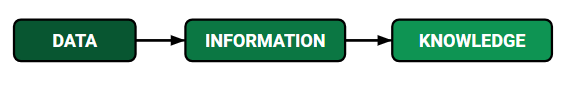
\includegraphics[width=0.8\textwidth]{DATA-1.png}
\end{frame}

\section{Questions About Data}

\begin{frame}
    \begin{itemize}
        \item \texttt{\color{red}Can the desired data be accessed?}\newline Before using data, ensure it is accessible, complies with legal, ethical, and financial considerations, and check for any agreements needed with data owners. Handle sensitive data carefully, removing personal identifiers when sharing. Consult legal experts to avoid future issues.
        \item \texttt{\color{red}Is the data volume sufficient?}\newline In machine learning, the required data volume is often uncertain, especially with strict performance criteria. Consider how quickly new data is generated—start with existing data, and allow new data to flow in during feature engineering, modeling, or other tasks. Use a representative subset for efficient training, and ensure it reflects the overall dataset characteristics.
    \end{itemize}
\end{frame}

\begin{frame}
    \begin{itemize}
        \item \texttt{\color{red}Is the data usable?} 
        \item Data  quality significantly affects model performance. Ensure the dataset is real, appropriately formatted (rows as samples, columns as features), and free of missing or duplicate values unless intended. Outdated data can limit model relevance, and incomplete datasets may lack diversity, affecting generalization.
        \item For example, the dataset might only include animals from a specific geographical region or images taken in a particular season, making it less representative of real-world scenarios.
    \end{itemize}
\end{frame}

\begin{frame}
    \begin{itemize}
        \item \texttt{\color{red}Is the data understandable?} 
        \item If the dataset is not fully understood, it can lead to errors during modeling. For instance, if the target variable is entirely calculable using one of the dataset features, but you are unaware of this relationship, it may result in misleading outcomes.
    \end{itemize}
\end{frame}

\begin{frame}
    \begin{itemize}{Data Leakage}
        \item Consider working on a house price prediction project where the model uses features like area, number of bedrooms, and neighborhood type. If you inadvertently include a feature like the real estate agent's commission—which has a direct relationship with the house price—this can cause \texttt{\color{red}data leakage}. The model might achieve near-perfect accuracy during training by exploiting this feature, but it will fail in real-world applications where such information isn’t available beforehand. Understanding the dataset thoroughly is essential to avoid such pitfalls..
    \end{itemize}
\end{frame}

\begin{frame}
    \begin{itemize}
        \item \texttt{\color{red}Is the data reliable?} 
        \item The reliability of data depends on the processes used for its collection. For instance, if labels are assigned by unwilling individuals or collected through sensors of questionable accuracy, their trustworthiness is debatable.

        \item Data reliability is also affected by delayed or indirect labeling. In delayed labeling, such as predicting customer retention 6 months ahead based on current behavior, significant intervening events may reduce label reliability. Indirect labeling, like inferring user interest in Instagram pages through actions like clicks or likes, can be misleading due to errors or external influences like advertisements. Ensuring data reliability is crucial for robust model performance.
    \end{itemize}
\end{frame}

\section{Data Challenges}


\begin{frame}{Labeling Samples}
    \begin{itemize}
        \item In supervised learning, labeled datasets are essential, but most available datasets are unlabeled. Consequently, a significant portion (around 80\%) of machine learning project time is spent collecting, organizing, and labeling data. Since manual labeling is resource-intensive, many teams rely on pre-labeled datasets.

        \item  example, to map business types in a city, buying data from a government body might be impractical due to incomplete or outdated records. Alternatively, you could collect images using camera-equipped vehicles and manually label businesses (e.g., cafés, gyms, pharmacies), though this approach is costly.

        \item Creative solutions include using software to streamline labeling or leveraging semi-supervised learning—manually label a small dataset to train a basic model and use it to label the rest, verified by human reviewers. This reduces the labeling burden significantly.

    \end{itemize}
\end{frame}


\begin{frame}{Data Quality}
    \begin{itemize}
        \item The quality of the dataset is one of the factors affecting model performance and consists of two main components:
        \item \texttt{\color{red}Raw Dataset Quality}
        \item \texttt{\color{red}Labeling Quality}
    \end{itemize}
\end{frame}

\begin{frame}
    \begin{itemize}
        \item Some common issues in raw datasets include the following, with some explained in this lesson and the last two covered in detail in future lessons:
        \item \texttt{\color{red}Noise}
        \item \texttt{\color{red}Bias}
        \item \texttt{\color{red}Low predictive power}
        \item \texttt{\color{red}Obsolescence}
        \item \texttt{\color{red}Outliers}
        \item \texttt{\color{red}Data Leakage}
    \end{itemize}
\end{frame}

\begin{frame}{Noise}
    \begin{itemize}
        \item A "noise" refers to a distorted or unrealistic sample. For example, a portion of an image may be missing, making it a noisy sample. Words in a text may be merged or improperly spaced, or there could be noise in audio data and similar issues. These types of data can often be partially corrected, such as recovering damaged images using specific algorithms. The problem of noisy data becomes more significant when the number of training samples is small (thousands or fewer). In such cases, noisy data can mislead the model's learning process. For instance, if there are 1,000 samples ranging between 0 and 10, along with three noisy samples exceeding 1,000, these three outliers can significantly skew the dataset's mean and variance.
    \end{itemize}
\end{frame}

\begin{frame}{Bias}
    \begin{itemize}
        \item Some common issues in raw datasets include the following, with some explained in this lesson and the last two covered in detail in future lessons:
        \item \texttt{\color{red}Selection Bias}
        \item \texttt{\color{red}Self-Selection Bias}
        \item \texttt{\color{red}Omitted Variable Bias}
        \item \texttt{\color{red}Sponsorship or Funding Bias}
        \item \texttt{\color{red}Sampling Bias}
    \end{itemize}
\end{frame}

\begin{frame}{Selection Bias}
    \begin{itemize}
        \item This occurs when a dataset is selected in a way that does not reflect the distribution of real-world data. This can happen due to ease of access to certain data sources or their cost-effectiveness. For example, imagine an author wants to know readers' opinions about their new book. The author sends the first few chapters to previous readers, who are likely to enjoy the new book because they already like the author's writing style. The key issue is that this information provides little insight into the opinion of a general reader about the new book.
    \end{itemize}
\end{frame}

\begin{frame}{Self-Selection Bias}
    \begin{itemize}
        \item In such cases, data is usually collected from sources that provide it voluntarily. Most survey datasets exhibit this kind of bias. For example, suppose you want to train a model to predict the behavior of successful entrepreneurs. You decide to first ask entrepreneurs whether they consider themselves successful and then keep only the data from those who claim to be successful. The issue is that genuinely successful entrepreneurs likely do not have time to answer your questions, while those who claim to be successful might be mistaken. Returning to the survey example, dissatisfied users are more inclined to give mid-range ratings instead of poor or very poor ones, causing the dataset to be biased toward mid-range ratings rather than the lower end.
    \end{itemize}
\end{frame}

\begin{frame}{Omitted Variable Bias}
    \begin{itemize}
        \item This occurs when the dataset lacks the necessary features for accurate predictions. For instance, imagine you are working on a predictive model to determine whether a customer will cancel their subscription within the next six months. You train a model that initially performs accurately. However, weeks after deployment, you observe unexpected results and a decline in model performance. Upon investigation, you discover that a new competitor is now offering very similar services at a much lower price. This feature was not available to your model initially, meaning it lacked critical information for accurate predictions.
    \end{itemize}
\end{frame}

\begin{frame}{Funding Bias}
    \begin{itemize}
        \item Imagine a company wants to use a model to predict successful AI companies in Iran over the next 10 years. Two AI companies volunteer to sponsor the project. They might expect their data in the model to be exaggerated to overstate their achievements. Such manipulation could compromise the model's performance and make it less effective than desired.
    \end{itemize}
\end{frame}

\begin{frame}{Sampling Bias}
    \begin{itemize}
        \item It is the responsibility of data scientists to ensure that the samples used to build a model align with the environment where the model will be deployed. This type of bias occurs when the distribution of the dataset used for training does not reflect the distribution of the input data the model will encounter in practical use.
    \end{itemize}
\end{frame}

\section{Data Splitting}
\begin{frame}{A Short Story}
    \begin{itemize}
        \item Let’s go through a scenario. Imagine you are a professor at TUMS, aiming to teach students the course material. Throughout the semester, you convey knowledge through lectures and course materials like books and notes. You also assign exercises for students to solve, helping them reinforce their understanding. If they make mistakes, they refer back to the notes to review and correct their errors.
    \end{itemize}
\end{frame}

\begin{frame}{A Short Story}
    \begin{itemize}
        \item At the semester's end, to determine which students have truly mastered the subject, you conduct a final exam with new questions. However, if you simply reuse questions from the notes or previous exercises, can you really identify who has genuinely learned the material? Definitely not!
    \end{itemize}
\end{frame}

\begin{frame}
    \begin{itemize}
        \item In machine learning, we follow a similar process. A portion of the dataset is provided to the model for learning (like books and notes). Another portion is used to verify the model's learning, and if needed, the training phase is repeated to ensure proper learning (like exercises and assignments). Finally, a completely unseen part of the dataset is used as the test data (exam questions). The error the model makes on the test data is considered its final error or final score.
    \end{itemize}
\end{frame}

\begin{frame}
    \begin{itemize}
        \item \texttt{\color{red}Training Set:} A portion of the dataset used for the model to learn.
        \item \texttt{\color{red}Validation Set:} A separate portion of the dataset not used during training but utilized to improve the model's performance.
        \item \texttt{\color{red}Test Set} A portion of the dataset used to evaluate the model's performance, serving as the final accuracy metric. This data should not be used during model development as it represents real-world examples.
    \end{itemize}
\end{frame}

\begin{frame}
    \centering
    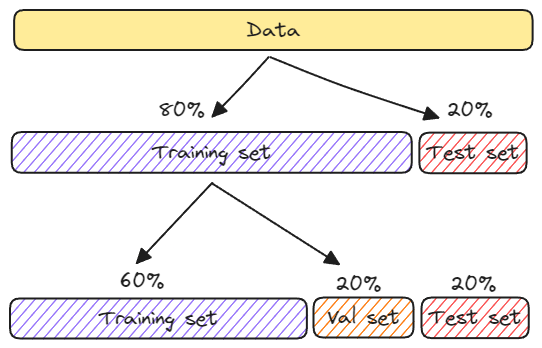
\includegraphics[width=0.8\textwidth]{Data-Spliting.png}
\end{frame}

\begin{frame}{Priority of Splitting:}
    \begin{itemize}
        \item The dataset should be split into training, validation, and test sets before applying any preprocessing. This prevents data leakage and ensures unbiased evaluation of the model.
    \end{itemize}
\end{frame}

\begin{frame}[fragile]{Implementing Using Sklearn}
	\begin{lstlisting}
from sklearn.model_selection import train_test_split

X_train, X_test, y_train, y_test = 
train_test_split(X, y, test_size=0.2, shuffle=True)

X_train, X_test, y_train, y_test = 
train_test_split(X, y, test_size=0.2, random_state=42)
       \end{lstlisting}
\end{frame}

\section{Outliers}
\begin{frame}
    \begin{itemize}
        \item An outlier is a data point that appears significantly different from most other samples in the dataset. Outliers can arise due to the following reasons:
    \end{itemize}
\end{frame}

\begin{frame}
    \begin{itemize}
        \item \texttt{\color{red}Error in data collection and recording:}Mistakes may occur during data collection, such as typos by human operators or system errors. For instance, in a dataset of housing prices in Beijing, a user might accidentally add an extra zero when recording the "price per square meter" of a house.

        \item \texttt{\color{red}Actual data distribution:}If outliers are not caused by errors, it indicates that the actual data distribution includes these deviations. For example, in the same housing dataset, luxurious and opulent homes in affluent areas of Beijing may naturally have prices significantly different from other properties.
    \end{itemize}
\end{frame}

\begin{frame}{Detecting Outliers}
    \begin{itemize}
        \item \texttt{\color{red}Statical Methods}
        \item \texttt{\color{red} Distance-Based Methods}
        \item \texttt{\color{red}Clustering-Based Methods}
    \end{itemize}
\end{frame}


\begin{frame}{Statical Methods}
    \begin{itemize}
        \item \texttt{\color{red}Z-Score:} This method calculates the standard deviation of the data points and identifies outliers as those with Z-scores exceeding a certain threshold (typically 3 or -3).
        \item \texttt{\color{red}Interquartile Range (IQR):} IQR identifies outliers as data points falling outside the range defined by Q1-k*(Q3-Q1) and Q3+k*(Q3-Q1), where Q1 and Q3 are the first and third quartiles, and k is a factor (typically 1.5).
    \end{itemize}
\end{frame}

\begin{frame}{IQR}
    \centering
    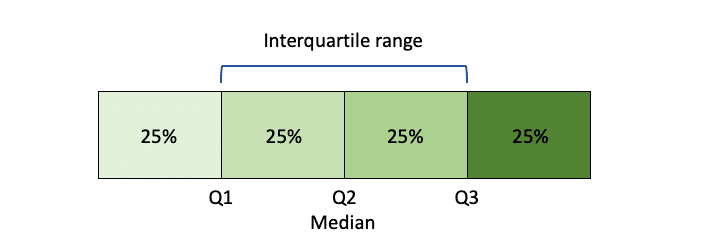
\includegraphics[width=0.8\textwidth]{iqr_quartiles.png}
\end{frame}

\begin{frame}{Box Plot}
    \centering
    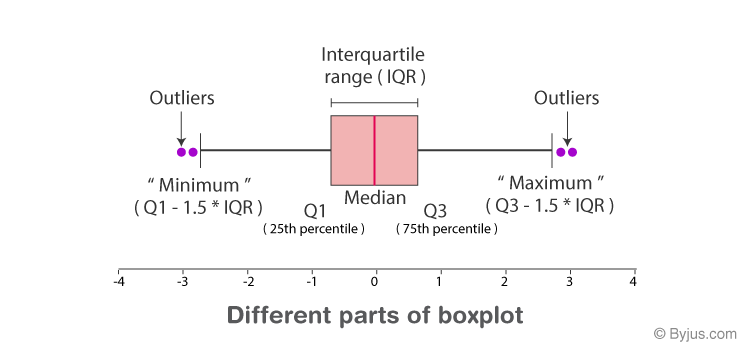
\includegraphics[width=0.8\textwidth]{Box-Plot.png}
\end{frame}

\begin{frame}{Techniques for Handling Outliers}
    \begin{itemize}
        \item \texttt{\color{red}1.Removal:} This involves identifying and removing outliers from the dataset before training the model. Common methods include:
        \item \texttt{\color{red}Threshold:} Outliers are identified as data points exceeding a certain threshold (e.g., Z-score > 3).
    \end{itemize}
\end{frame}

\begin{frame}{Techniques for Handling Outliers}
    \begin{itemize}
        \item \texttt{\color{red}2.Transformation:}This involves transforming the data to reduce the influence of outliers. Common methods include:
        \item \texttt{\color{red}Scaling:} Standardizing or normalizing the data to have a mean of zero and a standard deviation of one.
        \item \texttt{\color{red}Winterization} 
        \item \texttt{\color{red}Log transformation} 
    \end{itemize}
\end{frame}


\section{Missing Value}

\begin{frame}{What is a Missing Value ?}
    \begin{itemize}
        \item Missing values are data points that are absent for a specific variable in a dataset. They can be represented in various ways, such as blank cells, null values, or special symbols like “NA” or “unknown.” These missing data points pose a significant challenge in data analysis and can lead to inaccurate or biased results. 
    \end{itemize}
\end{frame}

\begin{frame}
    \centering
    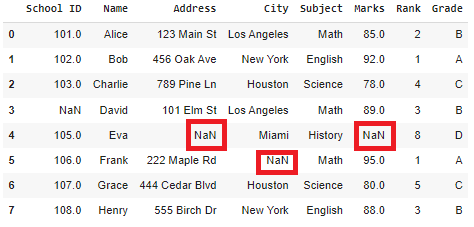
\includegraphics[width=0.8\textwidth]{m_v.png}
\end{frame}

\begin{frame}{Challenges}
    \begin{itemize}
        
    \end{itemize}
\end{frame}

\section{Imbalanced Data}


\begin{frame}
    \begin{center}
        {\Huge\ End of Data Preparation}
    \end{center}
\end{frame}

\end{document}

